% !TeX spellcheck = en_US
% !TeX encoding = utf8
% !TeX program = xelatex
% !BIB program = bibtex

\documentclass[notes]{beamer}
% \documentclass[draft]{beamer}	
\usetheme{Singapore}
% \usetheme{Hannover}
%\usepackage{pgfpages}
%\setbeameroption{show notes on second screen}

\usepackage[british]{babel}
\usepackage{graphicx,hyperref,url}
% \usepackage{ru}
\usepackage{mmstyles}
% \usepackage{hanging}
\usepackage{listings}
\usefonttheme[onlymath]{serif}
\usepackage{fontspec}
\usepackage{xeCJK}
% \pgfdeclareimage[width=\paperwidth,height=\paperheight]{bg}{background}
% \setbeamertemplate{background}{\pgfuseimage{bg}}
%% columns
\newcommand{\begincols}[1]{\begin{columns}{#1}}
\newcommand{\stopcols}{\end{columns}}
% \usepackage[backend=biber]{biblatex}
% \bibliography{./ref.bib}
%\addbibresource{ref.bib}
\usepackage{indentfirst}
\usepackage{longtable}
\usepackage{float}
%\usepackage{picins}
\usepackage{rotating}
\usepackage{subfigure}
\usepackage{tabu}
\usepackage{amsmath}
\usepackage{amssymb}
\usepackage{setspace}
\usepackage{amsfonts}
\usepackage{appendix}
\usepackage{listings}
\usepackage{xcolor}
\usepackage{geometry}
% \setCJKfamilyfont{cjkhwxk}{SimSun}
% \newcommand*{\cjkhwxk}{\CJKfamily{cjkhwxk}}
%\newfontfamily{\consolas}{Consolas}
%\newfontfamily{\monaco}{Monaco}
%\setmonofont[Mapping={}]{Consolas}	%英文引号之类的正常显示,相当于设置英文字体
%\setsansfont{Consolas} %设置英文字体 Monaco, Consolas,  Fantasque Sans Mono
% \setmainfont{Times New Roman}
% \newfontfamily{\consolas}{Times New Roman}
% \newfontfamily{\monaco}{Arial}
% \setCJKmainfont{Times New Roman}
%\setmainfont{MONACO.TTF}
%\setsansfont{MONACO.TTF}
\newcommand{\verylarge}{\fontsize{60pt}{\baselineskip}\selectfont}  
\newcommand{\chuhao}{\fontsize{44.9pt}{\baselineskip}\selectfont}  
\newcommand{\xiaochu}{\fontsize{38.5pt}{\baselineskip}\selectfont}  
\newcommand{\yihao}{\fontsize{27.8pt}{\baselineskip}\selectfont}  
\newcommand{\xiaoyi}{\fontsize{25.7pt}{\baselineskip}\selectfont}  
\newcommand{\erhao}{\fontsize{23.5pt}{\baselineskip}\selectfont}  
\newcommand{\xiaoerhao}{\fontsize{19.3pt}{\baselineskip}\selectfont} 
\newcommand{\sihao}{\fontsize{14pt}{\baselineskip}\selectfont}      % 字号设置  
\newcommand{\xiaosihao}{\fontsize{12pt}{\baselineskip}\selectfont}  % 字号设置  
\newcommand{\wuhao}{\fontsize{10.5pt}{\baselineskip}\selectfont}    % 字号设置  
\newcommand{\xiaowuhao}{\fontsize{9pt}{\baselineskip}\selectfont}   % 字号设置  
\newcommand{\liuhao}{\fontsize{7.875pt}{\baselineskip}\selectfont}  % 字号设置  
\newcommand{\qihao}{\fontsize{5.25pt}{\baselineskip}\selectfont}    % 字号设置 

\graphicspath{{./fig/}}

% \setbeamertemplate{footnote}{%
%   \hangpara{2em}{1}%
%   \makebox[2em][l]{\insertfootnotemark}\footnotesize\insertfootnotetext\par%
% }

\definecolor{cred}{rgb}{0.6,0,0}
\definecolor{cgreen}{rgb}{0.25,0.5,0.35}
\definecolor{cpurple}{rgb}{0.5,0,0.35}
\definecolor{cdocblue}{rgb}{0.25,0.35,0.75}
\definecolor{cdark}{rgb}{0.95,1.0,1.0}
\lstset{
	language=R,
	numbers=left,
	numberstyle=\tiny\color{black},
	keywordstyle=\color{cpurple}\consolas,
	commentstyle=\color{cgreen}\consolas,
	stringstyle=\color{cred}\consolas,
	frame=single,
	escapeinside=``,
	xleftmargin=1em,
	xrightmargin=1em, 
	backgroundcolor=\color{cdark},
	aboveskip=1em,
	breaklines=true,
	tabsize=3
} 

\providecommand{\tightlist}{%
  \setlength{\itemsep}{0pt}\setlength{\parskip}{0pt}}

  
% The title of the presentation:
%  - first a short version which is visible at the bottom of each slide;
%  - second the full title shown on the title slide;
\title[Opt for ML]{Multilayer Perceptrons (MLPs)}

% Optional: a subtitle to be dispalyed on the title slide
% \subtitle{Optimization for Machine Learning}

% The author(s) of the presentation:
%  - again first a short version to be displayed at the bottom;
%  - next the full list of authors, which may include contact information;
\author[YingmingLi]{Yingming Li \\ yingming@zju.edu.cn}
% The institute:
%  - to start the name of the university as displayed on the top of each slide
%    this can be adjusted such that you can also create a Dutch version
%  - next the institute information as displayed on the title slide

\institute[DSERC, ZJU]{Data Science \& Engineering Research Center, ZJU}

% Add a date and possibly the name of the event to the slides
%  - again first a short version to be shown at the bottom of each slide
%  - second the full date and event name for the title slide
\date[\today]{\today}

\begin{document}

\AtBeginSection[]
{
	\begin{frame}
		\frametitle{Outline}
		\tableofcontents[currentsection]
	\end{frame}
}

% \AtBeginSubsection[2-]
% {
%    \begin{frame}
%        \frametitle{Outline}
%        \tableofcontents[currentsection]
%    \end{frame}
% }
\begin{frame}
	\titlepage
	\begin{center}
		Adapted from slides provided by Prof.  Michael Mandel.		
	\end{center}
\end{frame}
\section{}\label{section}

\begin{frame}{Motivation}

\begin{itemize}
\tightlist
\item
  Multilayer networks are more powerful than single layer nets

  \begin{itemize}
  \tightlist
  \item
    \eg, XOR problem
  \end{itemize}
\end{itemize}

\centering 

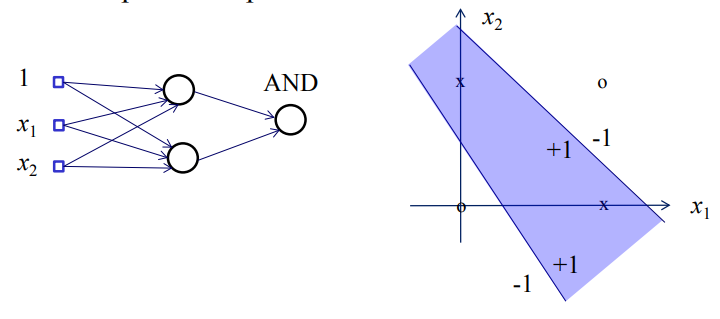
\includegraphics[width=0.70000\textwidth]{2018-03-10-11-05-54.png}\\

\end{frame}

\begin{frame}{Power of nonlinearity}

\begin{itemize}
\tightlist
\item
  For linear neurons, a multilayer net is equivalent to a single-layer
  net. This is not the case for nonlinear neurons

  \begin{itemize}
  \tightlist
  \item
    Why?
  \end{itemize}
\end{itemize}

\end{frame}

\begin{frame}{MLP architecture}

\centering 

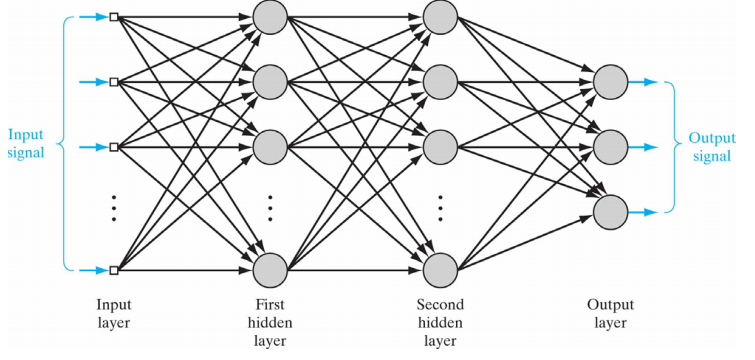
\includegraphics[width=0.80000\textwidth]{2018-03-10-11-08-20.png}\\

\end{frame}

\begin{frame}{Multi-layer perceptron}

\begin{itemize}
\tightlist
\item
  Think of an MLP as a complicated, non-linear function of its input
  parametrized by \(\vw\): \[\vy=F(\vx;\vw)\]
\item
  Note that ``Multi-layer perceptron'' is a bit of a misnomer because
  they use a continuous activation function
\end{itemize}

\end{frame}

\begin{frame}{MLP Training}

\begin{itemize}
\tightlist
\item
  Given a set of training data \(\{\vx_p,\vd_p\}\) can we adjust \(\vw\)
  so that the network is optimal
\item
  Optimal \wrt what criterion

  \begin{itemize}
  \tightlist
  \item
    Must define error criterion between \(\vy _\vp = F(\vx_\vp ; \vw)\)
    and \(\vd_p\)
  \item
    We will use the mean square error for now, but others are possible
    (and often preferable)
  \end{itemize}
\item
  Goal find \(\vw\) that minimizes
  \[  \bar{E}(\vw) = \sum_p E_p(\vw) = \sum_p \frac{1}{2} \|\vd_p - F(\vx_p ;\vw)\|^2\]
\end{itemize}

\end{frame}

\begin{frame}{Backpropagation}

\begin{itemize}
\tightlist
\item
  Because \(\bar{E} (\vw)\) is still a complication non-linear function,
  we will optimize it using gradient descent
\item
  Because of the structure of MLPs, we can compute the gradient of
  \(E_p (\vw)\) very efficiently using the backpropagation algorithm
\item
  Backpropagation computes the gradient of each layer recursively based
  on subsequent layers
\item
  Because this is \(E_p (\vw)\) and not \(\bar{E} (\vw)\), we will be
  using stochastic gradient descent
\end{itemize}

\end{frame}

\begin{frame}{Notation}

\begin{itemize}
\tightlist
\item
  Notation for one hidden layer (drop p for now)
\end{itemize}

\centering

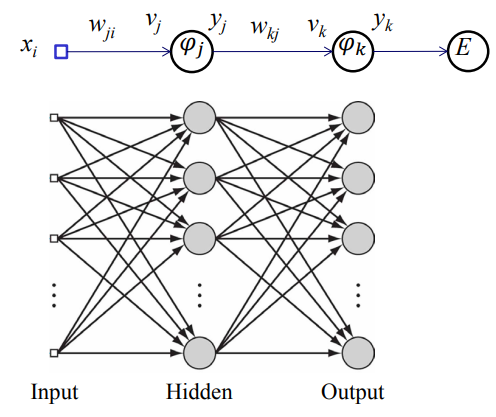
\includegraphics[width=0.70000\textwidth]{2018-03-10-13-48-45.png} ~

\end{frame}

\begin{frame}{Notation}

\begin{itemize}
\tightlist
\item
  Notation for one hidden layer (drop p for now)
\end{itemize}

\centering 

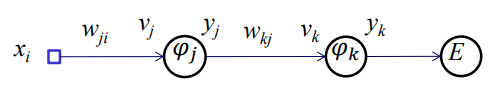
\includegraphics[width=0.70000\textwidth]{2018-03-10-13-49-42.png}\\

\begin{eqnarray*}
   y_k &=& \varphi_k \left(\sum_j w_{kj} \varphi_j \left(\sum_i w_{ji} x_i \right) \right) \\
   E(\vw) &=& 1/2 \sum_k (d_k - y_k)^2  
\end{eqnarray*}

\begin{itemize}
\tightlist
\item
  Keep in mind during the derivation:

  \begin{itemize}
  \tightlist
  \item
    How would changing \(E_p (\vw)\) affect the derivation
  \item
    How would changing \(\varphi (\vv)\) affect the derivation
  \end{itemize}
\end{itemize}

\end{frame}

\begin{frame}{Backprop}

\centering 

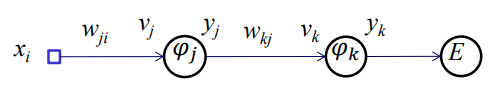
\includegraphics[width=0.70000\textwidth]{2018-03-10-13-49-42.png}\\

\begin{align} 
    y & = \frac{1}{2} \sum_k (d_k - y_k)^2 \\ %\nonumber
      & =  \frac{1}{2}\sum_k \left(
        d_k - \underbrace{\varphi_k 
        \left( \overbrace{\sum_j w_{kj} y_j}^{v_k} \right)
         }_{y_k}
      \right)^2 
\end{align}

\begin{itemize}
\tightlist
\item
  Then, to adjust the hidden-output weights
\end{itemize}

\begin{equation}
    \frac{\partial }{\partial w_{kj}} E(\vw) = 
    \textcolor{red}{
        \frac{\partial E}{\partial y_k}} 
    \textcolor{blue}{
        \frac{\partial y_k}{\partial v_k}
    } 
    \textcolor{green}{
        \frac{\partial v_k}{\partial w_{kj}}
    }
\end{equation}

\end{frame}

\begin{frame}{Backprop}

\begin{align}
    \textcolor{red}{
    \frac{\partial E}{\partial y_k}} & = -(d_k - y_k) = -e_k                                           \\
    \textcolor{blue}{
        \frac{\partial y_k}{\partial v_k}
    }                                & = \frac{\partial }{\partial v_k} \varphi (v_k) = \varphi ' (v_k) \\
    \textcolor{green}{
        \frac{\partial v_k}{\partial w_{kj}}
    }                                & = y_j
\end{align}

So

\begin{equation}
  \frac{\partial }{\partial w_{kj}} E(\vw) = 
    \textcolor{red}{
        \frac{\partial E}{\partial y_k}} 
    \textcolor{blue}{
        \frac{\partial y_k}{\partial v_k}
    } 
    \textcolor{green}{
        \frac{\partial v_k}{\partial w_{kj}}
    } = -e_k \varphi ' (v_k) y_j 
\end{equation}

\end{frame}

\begin{frame}{Backprop}

\centering 

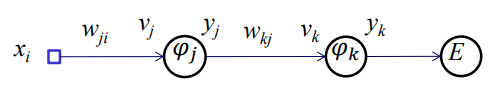
\includegraphics[width=0.70000\textwidth]{2018-03-10-13-49-42.png}\\

\begin{itemize}
\tightlist
\item
  Hence, to update the hidden-output weights
\end{itemize}

\begin{align}
    w_{kj} (n+1 ) & = w_{kj} (n) - \eta \frac{\partial E}{\partial w_{kj}} \\
    &= w_{kj} (n) + \eta \underbrace{ e_k \varphi ' (v_k)  }_{\delta_k} y_j  \\ 
    &= w_{kj}(n) + \eta \delta_k y_j \quad (\delta \textrm{ rule }) 
\end{align}

\end{frame}

\begin{frame}{Backprop}

\centering 

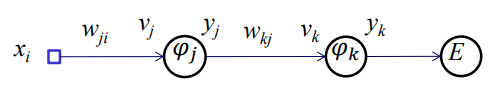
\includegraphics[width=0.70000\textwidth]{2018-03-10-13-49-42.png}\\

\begin{itemize}
\tightlist
\item
  For the input-hidden weights,
\end{itemize}

\begin{equation}
  \frac{\partial }{\partial w_{ji}} E(\vw) = 
    \textcolor{red}{
        \frac{\partial E}{\partial y_j}} 
    \textcolor{blue}{
        \frac{\partial y_j}{\partial v_j}
    } 
    \textcolor{green}{
        \frac{\partial v_j}{\partial w_{ji}}
    }
\end{equation}

\begin{align}
    \textcolor{red}{
        \frac{\partial E}{\partial y_k}
    } & = - \sum_{k}(d_k - y_k) \varphi ' (v_k) w_{kj} \\
    \textcolor{blue}{
        \frac{\partial y_k}{\partial v_k}
    } & = \varphi ' (v_j)                               \\
    \textcolor{green}{
        \frac{\partial v_k}{\partial w_{ji}}
    } & = x_i
\end{align}

\end{frame}

\begin{frame}{Backprop}

\centering 

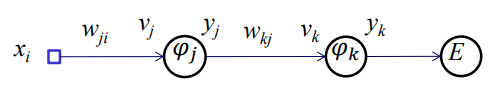
\includegraphics[width=0.70000\textwidth]{2018-03-10-13-49-42.png}\\

\begin{itemize}
\tightlist
\item
  So\\

  \begin{align}
  \frac{\partial }{\partial w_{ji}} E(\vw) &= 
    \textcolor{red}{
        \frac{\partial E}{\partial y_j}} 
    \textcolor{blue}{
        \frac{\partial y_j}{\partial v_j}
    } 
    \textcolor{green}{
        \frac{\partial v_j}{\partial w_{ji}}
    } \\
    &=  - \sum_{k} \underbrace{(d_k - y_k) \varphi ' (v_k) }_{\delta_k} w_{kj} \varphi ' (v_j) x_i  \\
    & = -(\underbrace{\sum_k \delta_k w_{kj}}_{e_j}) \varphi ' (v_j) x_i \\ 
    &= -e_j \varphi ' (v_j )x_i
  \end{align}
\end{itemize}

\end{frame}

\begin{frame}{Backprop}

\centering 

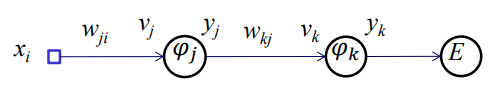
\includegraphics[width=0.70000\textwidth]{2018-03-10-13-49-42.png}\\

\begin{itemize}
\tightlist
\item
  Hence, to update the input-hidden weights
\end{itemize}

\begin{align}
    w_{ji} (n+1 ) & = w_{ji} (n) - \eta \frac{\partial E}{\partial w_{ji}} \\
    &= w_{ji} (n) + \eta \underbrace{ e_j \varphi ' (v_j)  }_{\delta_j} x_i  \\ 
    &= w_{ji}(n) + \eta \delta_j x_i   
\end{align}

\begin{itemize}
\tightlist
\item
  The above is called the generalized rule
\end{itemize}

\end{frame}

\begin{frame}{Backprop}

\begin{figure}
\centering
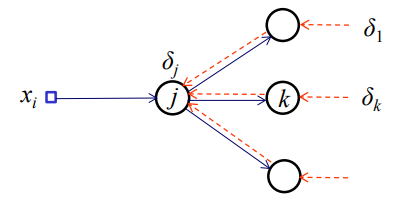
\includegraphics[width=0.50000\textwidth]{2018-03-10-15-36-58.png}
\caption{Illustration of the generalized rule}
\end{figure}

\begin{itemize}
\tightlist
\item
  The generalized rule gives a solution to the credit (blame) assignment
  problem
\end{itemize}

\end{frame}

\begin{frame}{Hyperbolic tangent function}

\centering 

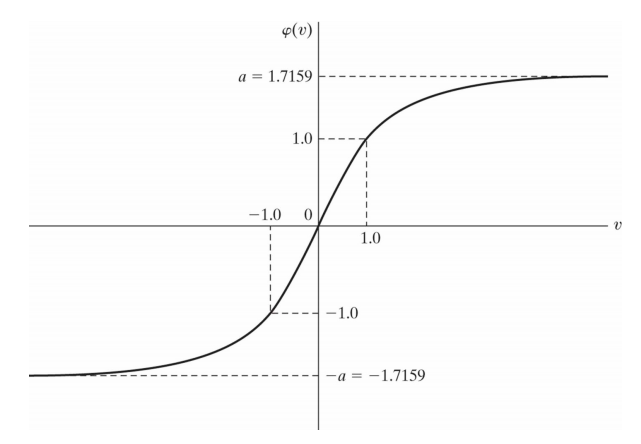
\includegraphics[width=0.80000\textwidth]{2018-03-10-15-37-41.png} ~

\end{frame}

\begin{frame}{Backprop}

\centering 

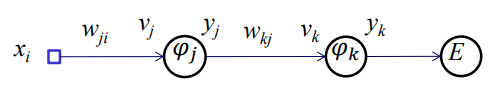
\includegraphics[width=0.70000\textwidth]{2018-03-10-13-49-42.png}\\

\begin{itemize}
\tightlist
\item
  For the logistic sigmoid activation, we have
\end{itemize}

\[\varphi ' ( v ) = a \varphi ( v )[1 -\varphi  ( v )]\]

\begin{itemize}
\tightlist
\item
  hence
\end{itemize}

\begin{align}
    \delta_ k & = e_k [ay_k (1 - y_k )]                       \\
              & = ay_k [1 - y_k ][d_ k - y_k ]                \\
    \delta_j  & = ay_ j [1 - y _j ]  \sum_{k} w_{kj} \delta_k
\end{align}

\end{frame}

\begin{frame}{Backprop}

In summary:

\begin{align}
    \frac{\partial }{\partial w_{kj} } E(\vw) & =   -e_k \varphi ' (v_k) y_j \\
    \frac{\partial }{\partial w_{ji}} E(\vw)  & =   -e_j \varphi ' (v_j) x_i
\end{align}

\begin{itemize}
\tightlist
\item
  Backprop learning is local, concerning ``presynaptic'' and
  ``postsynaptic'' neurons only
\item
  How would changing \(E(\vw)\) affect the derivation
\item
  How would changing \(\varphi (\vv)\) affect the derivation
\end{itemize}

\end{frame}

\begin{frame}{Backprop illustration}

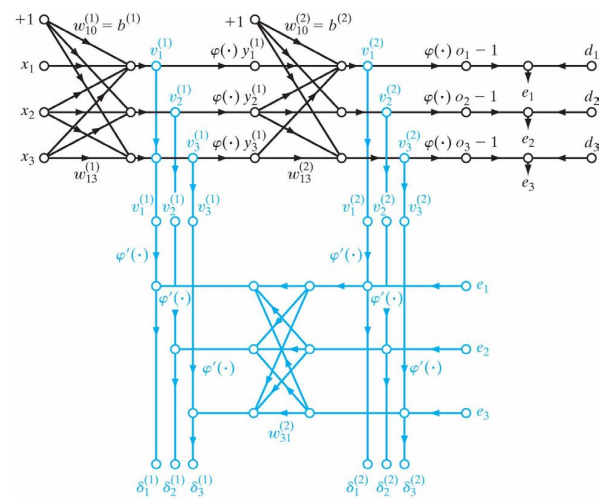
\includegraphics[width=0.80000\textwidth]{2018-03-10-15-46-32.png} ~

\end{frame}

\begin{frame}{Backprop}

\begin{itemize}
\tightlist
\item
  Extension to more hidden layers is straightforward. In general we have
  \[ \Delta w_ {ji} (n) = \eta \delta _j y_i\]

  \begin{itemize}
  \tightlist
  \item
    The rule applies to the output layer and the generalized rule
    applies to hidden layers, layer by layer from the output end.
  \item
    The entire procedure is called backpropagation (error is back
    propagated from the outputs to the inputs)
  \end{itemize}
\end{itemize}

\end{frame}

\begin{frame}{MLP design parameters}

\begin{itemize}
\tightlist
\item
  Several parameters to choose when designing an MLP (best to evaluate
  empirically)
\item
  Number of hidden layers
\item
  Number of units in each hidden layer
\item
  Activation function
\item
  Error function
\end{itemize}

\end{frame}

\begin{frame}{Universal aproximation theorem}

\begin{itemize}
\tightlist
\item
  MLPs can learn to approximate any function, given sufficient layers
  and neurons (an existence proof)
\item
  At most two hidden layers are sufficient to approximate any function.
  One hidden layer is sufficient for any continuous function
\end{itemize}

\end{frame}

\begin{frame}{Optimization tricks}

\begin{itemize}
\tightlist
\item
  For a given network, local minima of the cost function are possible
\item
  Many tricks exist to try to find better local minima

  \begin{itemize}
  \tightlist
  \item
    Momentum: mix in gradient from step \(n - 1\)
  \item
    Weight initialization: small random values
  \item
    Stopping criterion: early stopping
  \item
    Learning rate annealing: start with large \(\eta\) , slowly shrink
  \item
    Second order methods: use a separate \(\eta\) for each parameter or
    pair of parameters based on local curvature
  \item
    Randomization of training example order
  \item
    Regularization, i.e., terms in \(E(w)\) that only depend on \(w\)
  \end{itemize}
\end{itemize}

\end{frame}

\begin{frame}{Learning rate control: momentum}

\begin{itemize}
\item
  To ease oscillating weights due to large , some inertia (momentum) of
  weight update is added
  \[     \Delta   w_{ji} (n) = \eta \delta_ j y_i + \alpha \Delta w_ {ji} (n - 1),                        0 < \alpha < 1\]

  \begin{itemize}
  \tightlist
  \item
    In the downhill situation,
    \(\Delta w_ {ji} (n)\approx \frac{\eta}{1-\alpha} \delta _ j y_i\)

    \begin{itemize}
    \tightlist
    \item
      thus accelerating learning by a factor of \(1/(1 - \alpha )\)
    \end{itemize}
  \item
    In the oscillating situation, it smooths weight change, thus
    stabilizing oscillations
  \end{itemize}
\end{itemize}

\end{frame}

\begin{frame}{Weight initialization}

\begin{itemize}
\tightlist
\item
  To prevent saturating neurons and break symmetry that can stall
  learning, initial weights (including biases) are typically randomized
  to produce zero mean and activation potentials away from saturation
  parts of the activation function

  \begin{itemize}
  \tightlist
  \item
    For the hyperbolic tangent activation function, avoiding saturation
    can be achieved by initializing weights so that the variance equals
    the reciprocal of the number of weights of a neuron
  \end{itemize}
\end{itemize}

\end{frame}

\begin{frame}{Stopping criterion}

\begin{itemize}
\tightlist
\item
  One could stop after a predetermined number of epochs or when the MSE
  decrease is below a given criterion
\item
  Early stoping with cross validation: keep part of the training set,
  called validation subset, as a test for generalization performance
\end{itemize}

\centering 

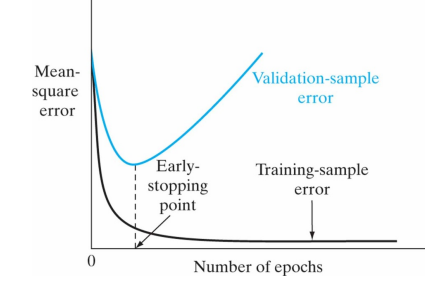
\includegraphics[width=0.50000\textwidth]{2018-03-10-16-00-59.png} ~

\end{frame}

\begin{frame}{Selecting model parameters: cross validation}

\begin{itemize}
\tightlist
\item
  Must have separate training, validation, and test datasets to avoid
  over-confidence, over-fitting
\item
  When lots of data is available, have dedicated sets
\item
  When data is scarce, use cross-validation

  \begin{itemize}
  \tightlist
  \item
    Divide the entire training sample into an estimation subset and a
    validation subset (e.g.~80/20 split)
  \item
    Rotate through 80/20 splits so that every point is tested on once
  \end{itemize}
\end{itemize}

\end{frame}

\begin{frame}{Cross validation illustration}

\centering 

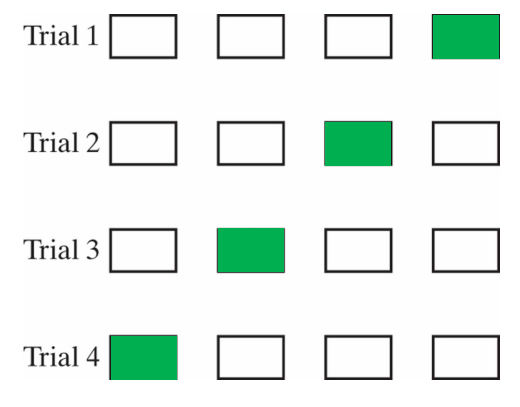
\includegraphics[width=0.60000\textwidth]{2018-03-10-16-01-35.png} ~

\end{frame}

\begin{frame}{MLP applications}

\begin{itemize}
\tightlist
\item
  Task: Handwritten zipcode recognition (1989)
\item
  Network description

  \begin{itemize}
  \tightlist
  \item
    Input: binary pixels for each digit
  \item
    Output: 10 digits
  \item
    Architecture: 4 layers (16x16-12x8x8-12x4x4-30-10)
  \end{itemize}
\item
  Each feature detector encodes only one feature within a local input
  region. Different detectors in the same module respond to the same
  feature at different locations through weight sharing. Such a layout
  is called a convolutional net
\end{itemize}

\end{frame}

\begin{frame}{Zipcode recognizer architecture}

\begin{figure}
\centering
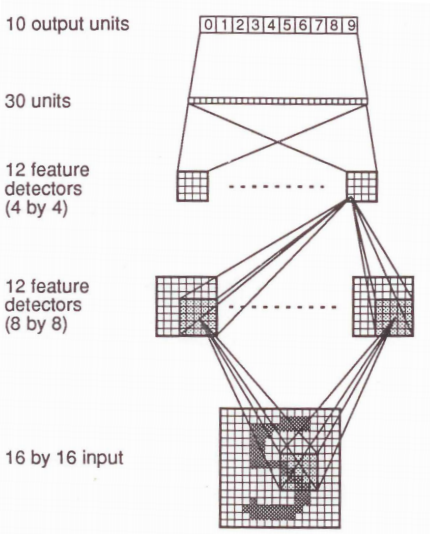
\includegraphics[width=0.50000\textwidth]{2018-03-10-16-07-59.png}
\caption{zipcode recognizer architecture}
\end{figure}

\end{frame}

\begin{frame}{Zipcode recognition (cont.)}

\begin{itemize}
\tightlist
\item
  Performance: trained on 7300 digits and tested on 2000 new ones

  \begin{itemize}
  \tightlist
  \item
    Achieved 1\% error on the training set and 5\% error on the test set
  \item
    If allowing rejection (no decision), 1\% error on the test set
  \item
    The task is not easy (see a handwriting example)
  \end{itemize}
\item
  Remark: constraining network design is a way of incorporating prior
  knowledge about a specific problem

  \begin{itemize}
  \tightlist
  \item
    Backprop applies whether or not the network is constrained
  \end{itemize}
\end{itemize}

\end{frame}

\begin{frame}{Letter recognition example}

\begin{itemize}
\tightlist
\item
  The convolutional net has been subsequently applied to a number of
  pattern recognition tasks with state-of-the-art results

  \begin{itemize}
  \tightlist
  \item
    Handwritten letter recognition
    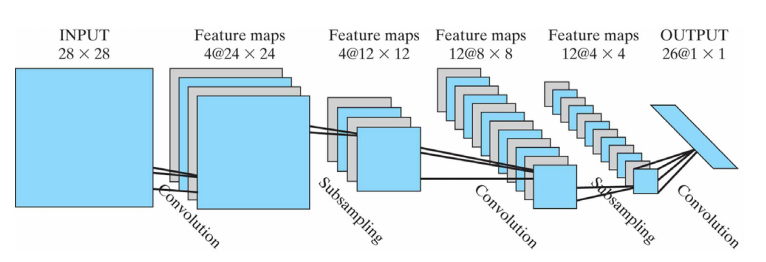
\includegraphics[width=0.80000\textwidth]{2018-03-10-16-09-17.png}
  \end{itemize}
\end{itemize}

\end{frame}

\begin{frame}{Automatic driving}

\begin{itemize}
\tightlist
\item
  ALVINN (automatic land vehicle in a neural network)
  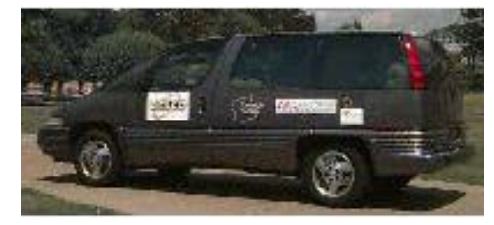
\includegraphics[width=0.80000\textwidth]{2018-03-10-16-09-46.png}

  \begin{itemize}
  \tightlist
  \item
    One hidden layer, one output layer
  \item
    Five hidden nodes, 32 output nodes (steer left - steer right)
  \item
    960 inputs (30 x 32 image intensity array)
  \item
    5000 trainable weights
  \end{itemize}
\item
  Later success of Stanley (won \$ 2M DARPA Grand Challenge in 2005)
\end{itemize}

\end{frame}

\begin{frame}{Other MLP applications}

\begin{itemize}
\tightlist
\item
  NETtalk, a speech synthesizer
\item
  GloveTalk, which converts hand gestures to speech
\end{itemize}

\end{frame}
\begin{frame}
	\chuhao Thank you! %\fontspec{LHANDW.TTF}
\end{frame}
\end{document}
